%
% main.tex -- Paper zum Thema <elektro>
%
% (c) 2020 Autor, OST Ostschweizer Fachhochschule
%
% !TEX root = ../../buch.tex
% !TEX encoding = UTF-8
%
\chapter{Zweidimensionale Elektrostatik 
\label{chapter:elektro}}
\kopflinks{Zweidimensionale Elektrostatik}
\begin{refsection}
\chapterauthor{Malenka Hossli und Andrea Studer}

\index{Malenka Hossli}%
\index{Hossli, Malenka}%
\index{Andrea Studer}%
\index{Studer, Andrea}%

%
% einleitung.tex -- Beispiel-File für die Einleitung
%
% (c) 2020 Prof Dr Andreas Müller, Hochschule Rapperswil
%
% !TEX root = ../../buch.tex
% !TEX encoding = UTF-8
%

\section{Einleitung}
In diesem Kapiteln wird beschrieben, was unter zweidimensionaler Elektrostatik verstanden wird, welche physikalischen und mathematischen Gesetze ihr zugrunde liegen und wie diese zur Berechnung und Darstellung elektrostatischer Felder eingesetzt werden können.
Ausgehend vom Coulomb-Gesetz werden das elektrische Feld und das elektrische Potential eingeführt und deren Zusammenhang beschrieben. 
Dabei wird betrachtet, wie sich elektrische Felder und Potentiale im zweidimensionalen Raum darstellen lassen und welche Eigenschaften ihre Feld- und Äquipotentiallinien haben.
Weiter wird erörtert, wie diese Grössen mithilfe komplexer Funktionen beschrieben werden können. 
Dies dient als mathematische Grundlage, um elektrostatische Probleme nicht nur für einfache Geometrien wie den Kreis, sondern auch für kompliziertere Formen zu beschreiben.
Es wird der Riemannsche Abbildungssatz vorgestellt und erläutert, wie wie verschiedene Geometrien auf einfachere Gebiete abgebildet werden, für welche das elektrische Feld und das Potential bereits bekannt sind. 
Am Beispiel des Kreises und später mithilfe der Schwarz-Christoffel-Transformation wird gezeigt, wie dieses Prinzip auf verschiedene Geometrien angewendet werden kann.

Bevor wir in das Kapitel einsteigen, mögen einige Beispiel zur Anschauung dienen: 
Elektrostatik wird für uns Menschen erfahrbar, wenn es zu Ladungstrennungen kommt.
Blitze, klebende Styroporkügelchen und und als Sonderbeispiel Van de Graaff Bandgeneratoren --- Grundlage für diese physikalischen Phänomene ist folgendes Prinzip:
Gleichartige Ladungen stossen sich ab, ungleichartige Ladungen ziehen sich an.
Beispielsweise wenn wir einen synthetischen Pullover über den Kopf ziehen und dabei ein Knistern hören. Berühren wir dann einen anderen (geerdeten) Menschen, funkt es.
Ein kurzes Zwicken beweist die unsichtbare elektrostatische Aufladung, die durch Reibung des Pullovers erzeugt worden ist.
Als Fachpersonen im Bereich der Elektrotechnik haben wir häufig Bauteile in der Hand, die wir vor elektrostatischer Entladung (ESD) schützen müssen.
Zum Schutz solcher empfindlicher Bauteile tragen wir daher geerdete Armbänder, was Ladungstrennung, welche zu ESD führt, verhindert. 

Um elektrostatische Aufladung zu demonstrieren, wird eine (langhaarige) Versuchsperson daher zuallererst auf ein isoliertes Podest gestellt.
Ladung, die durch den von Robert Van de Graaff 1929 erfundenen Generator auf eine Metallkugel gebracht wird, gelangt mittels Berührung der Handflächen auf die Versuchsperson.
%\textcolor{red}{TODO Foto Versuchsperson mit Feldlinien eingezeichnet}
Der Van de Graaff Generator nutzt die mechanische Reibung eines Gummibandes, um gleichartige Ladungsträger auf einer Metallkugel abzuladen, welche sich anschliessend durch Influenz auf der ganzen Oberfläche verteilen.
Es spielt dabei keine Rolle, ob die Ladungsträger positiv oder negativ sind.
Die Ladungen wandern auf die Versuchsperson, und da sie sich abstossen, entsteht eine kleine Kraft.
Diese reicht bei genügend trockener Luft aus, um die Haare der Versuchsperson zu Berge stehen zu lassen.
Trotz seines tiefen Wirkungsgrades kommt der Van de Graaff Generator zur Erzeugung hoher Gleichspannungen als Teilchenbeschleuniger zum Einsatz \cite{elektro:lexikon}.

% In diesem Kapitel werden die Zusammenhänge zwischen Elektrostatik und Geometrie beschrieben. 
% Die Geometrie wird auf zwei Dimensionen reduziert, was zu Vereinfachungen führt.
% Die prominenteste Vereinfachung ist, dass von den vier Maxwell-Gleichungen nur noch eine relevant ist, nämlich die Laplace Gleichung (\ref{elektro:equation:laplace}) für das Potential. 
% Der Fokus liegt auf dem Zusammenhang zwischen elektrischen Feldlinien und Äquipotentiallinien im zweidimensionalen Raum.
% Feldlinien und Potential werden als komplexe Funktionen interpretiert und über komplexe Abbildungen miteinander verknüpft.
% Wie das funktioniert, wird anhand von vielen Beispielen in diesem Kapitel erklärt, bewiesen und veranschaulicht. 


\section{Grundlagen der Elektrostatik\label{elektro:section:EFeld}}
\kopfrechts{Grundlagen der Elektrostatik}
Das Begriff Elektrostatik enthält zwei grundlegende Begriffe: Elektrizität und Statik. 
Es fliesst aber kein Strom, es werden ausschliesslich ruhende elektrische Ladungsträger betrachtet.
In unseren Anwendungen verteilen sich diese Ladungen auf der Oberfläche von leitenden Körpern, bis die Kräfte zwischen den Ladungen einen stabilen Zustand erreicht haben, und still stehen bleiben.
Dann spricht man von Elektrostatik, denn die Ladungen bewegen sich nicht mehr, sie sind statisch. Wird nach der Zeit abgeleitet, um die Änderung über die Zeit zu sehen, so ist die Ableitung
$\frac{\partial \vec{E}}{\partial t} = 0$
gleich Null. 

\subsection{Vektor- und Skalarfeld, Quellenfeld und Homogenität
\label{elektro:subsection:VektorSkalar}}
Das \textbf{elektrische Feld} ist ein Vektorfeld.
Das bedeutet, jedem Punkt im Raum wird ein Vektor mit einem Betrag und einer Richtung der elektrischen Feldstärke zugeordnet. 
Die Länge des Vektors zeigt, wie stark das elektrische Feld an diesem Punkt ist. 
Seine Richtung ist diejenige Richtung, in die eine Probeladung bewegt wird, wenn sie an diesem Punkt platziert würde.
Eine Probeladung ist eine Ladung, die so klein ist, dass sie das Feld nicht beeinflusst.
Sie ist nur da um die Stärke des Feldes zu messen, ist also nur ein Werkzeug und keine physische Ladung.
Das \textbf{Potentialfeld} ist ein Skalarfeld.
Jedem Punkt im Raum wird nur der Betrag, also nur die Stärke des Potentials zugeordnet, aber keine Richtung.
Diese Stärke wird in Volt angegeben, das ist die definiere Einheit für das Potential.

Elektrostatische Felder sind Quellenfelder, das bedeutet, es gibt einen Punkt, von dem alle Feldlinien ausgehen oder auf den alle Feldlinien zulaufen. 
Es hat keine Wirbel, die Pfeile sind somit nicht in eine Richtung gebogen, sondern immer gerade.
Es ergeben sich also keine geschlossenen Feldlinien, die in sich selbst enden (wie es zum Beispiel beim Magnetfeld der Fall ist).
Die Feldlinien des elektrostatischen Felds beginnen immer auf positiven Ladungen und enden auf negativen. 
Die Feldlinien können sich aber im Unendlichen schliessen, somit laufen die Feldlinien einfach radial bis ins Unendliche.

Verlaufen die Feldlinien parallel, spricht man von einem homogenen Feld, ansonsten von einem inhomogenen Feld.
Das Feld zwischen zwei parallelen Kondensatorplatten beispielsweise ist homogen, was die mathematische Berechnung erheblich erleichtert. 

\subsection{Das Coulomb-Gesetz
\label{elektro:subsection:Coulomb}}
Das Coulomb-Gesetz
\begin{equation}
	\vec{F} = \frac{Q_1 Q_2}{4\pi\varepsilon_0 R^{2}}\hat{R}
	\label{equation:Coulomb}
\end{equation}
beschreibt die Kraft, die zwei ruhende Punktladungen aufeinander ausüben.
Eine Punktladung ist eine punktsymmetrische Ladung ohne räumliche Ausdehnung.
In der Praxis ist das Coulomb-Gesetz nur gültig, wenn der Abstand zwischen den beiden Ladungen viel grösser ist als die Ausdehnung der Ladungen selbst.
Ist dies nicht der Fall, werden sich andere physikalische Effekte bemerkbar machen, die das Coulomb-Gesetz nicht berücksichtigt.
Die Coulomb-Kraft hängt von der Grösse der jeweiligen Ladung $Q_1$ und $Q_2$ ab.
Werden die Ladungen grösser, so nimmt auch die Kraft zu.
Der Abstand zwischen den beiden Ladungen ist der bestimmende Faktor, da die Kraft mit dem Quadrat des Abstands $R$ zwischen den Ladungen abnimmt.
$\vec{R} = R \cdot \hat{R}$ ist der Distanzvektor zwischen den Ladungen und muss immer vom Ort der Ursache auf den Ort der Wirkung zeigen, damit die resultierenden Kräfte die korrekte Richtung aufweisen.
$\hat{R}$ ist in der Elektrotechnik der Einheitsvektor der Länge 1 und Richtung von $\vec{R}$.
Liegt einer der Punkte im Ursprung wird die Variable $r$ verwendet, dies ist wichtig für das Verstehen der später hergeleiteten Formeln.
Die beiden Komponenten des Vektors sind der Betrag $R$ und die Richtung $\hat{R}$, diese werden in der Formel \eqref{equation:Coulomb} separat verwendet.
Weitere wichtige Definitionen:
\begin{itemize}
	\item Das Coulomb-Gesetz gilt für Distanzen zwischen $10^{-16}$ und $10^{8}$ Metern. 
	\item Für $R = 0$ ist es nicht definiert. 
	\item $\varepsilon_0$ ist die elektrische Permittivität des Vakuums und beträgt ungefähr 8.854 pF/m. 
\end{itemize}

\subsection{Das elektrische Feld}
Im ersten Abschnitt \ref{elektro:section:EFeld} wurde das elektrische Feld als Vektorfeld definiert.
Es geht nun darum, das E-Feld auch mathematisch zu definieren.
Das elektrische Feld und die Coulomb-Kraft sind über die Normierung auf die Probeladung q
\begin{equation}
	\vec{E} = \frac{\vec{F}}{q} = \frac{\text{Kraft}}{\text{Probeladung}} = \frac{Q}{4\pi\varepsilon_0 r^{2}}\hat{r}
	\label{elektro:equation:EFeld}
\end{equation}
\begin{figure}
	\centering
	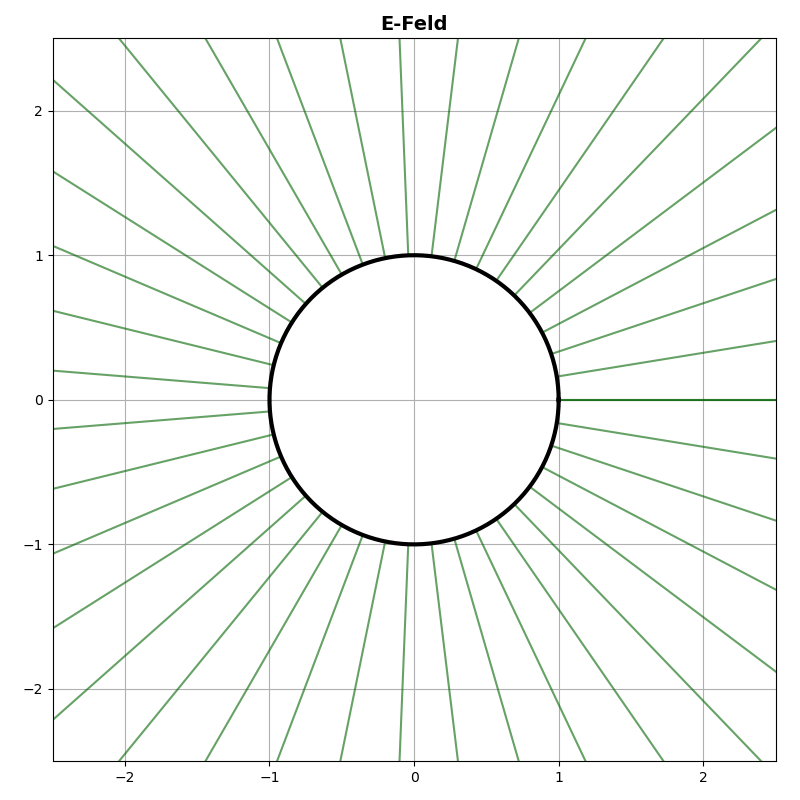
\includegraphics[width=0.9\linewidth]{papers/elektro/grafik/e_feld_kreis.png}
	\label{elektro:figure:e_feld}
	\caption[]{Normiert auf eine Punktladung q handelt es sich beim elektrischen Feld um ein Radialfeld.}
\end{figure}
verwandt.
Bringt man eine Probeladung $q$ in die Nähe einer Punktladung $Q$, so ist die Kraft, welche auf die Probeladung wirkt, als elektrische Feldstärke definiert.
Die Kraft ist das gesamte vektorielle Kraftfeld, das an der jeweiligen Stelle auf $q$ wirkt, und wird in Volt pro Meter angegeben $[\vec{E}] = V/m$.
Es handelt sich um ein Radialfeld (ausgehend von der positiven und führend zur negativen Quelle).

\subsection{Das elektrische Potential $\varphi$
\label{elektro:subsection:Potential}}
Genau wie beim $\vec{E}$-Feld, das durch Normalisierung der Coulomb-Kraft mit einer Probeladung definiert wird, ist das elektrische Potential wie folgt
\begin{equation}
	\varphi = \frac{W}{q} = \frac{Q}{4\pi\varepsilon_0r} = - \int_{\text{Pref}}^P \vec{E} \cdot d\vec{l}
	\label{elektro:equation:Potential}
\end{equation}
durch Normalisierung der Energie $W$ mit einer Probeladung definiert.

Die Einheit von $\varphi$ ist Volt $[\varphi] = V$, und ist wie am Anfang erwähnt ein Skalarfeld.
Somit ist jedem Punkt ein Betrag zugeordnet, und mit Beträgen kann eine Differenz zwischen zwei Punkten im Skalarfeld gebildet werden.
Diese Differenz zwischen zwei Potentialen ist die Spannung, es wird dabei oft ein Referenzpunkt gewählt, der als Nullpunkt dient.
%Aus dem Potential jedes einzelnen Punktes kann die elektrische Feldstärke berechnet werden.
Das negative Vorzeichen in der Formel \eqref{elektro:equation:Potential} hat seinen Ursprung in der Wahl des Bezugssystem, der Referenz Ref, von wo aus integriert wird.
In der Formel \ref{elektro:equation:Potential} wird der Betrag des elektrostatischen Felds $E$ als Variable verwendet, das an jedem Punkt von $E$ auf das dort herrschende Potential geschlossen werden kann und umgekehrt. 
Wenn auf zwei nebeneinanderliegenden Punkten dasselbe Potential $\varphi$ herrscht, werden diese mit einer Linie verbunden, der sogenannten Äquipotentiallinie.
Diese Linien sind immer geschlossen und verlaufen senkrecht zu den E-Feldlinien.
Sie haben aber noch eine weitere wichtige Eigenschaft:
Auf diesen Linien kann eine Probeladung beliebig verschoben werden, ohne dass dabei Arbeit aufgewandt werden muss.
\begin{figure}
	\centering
	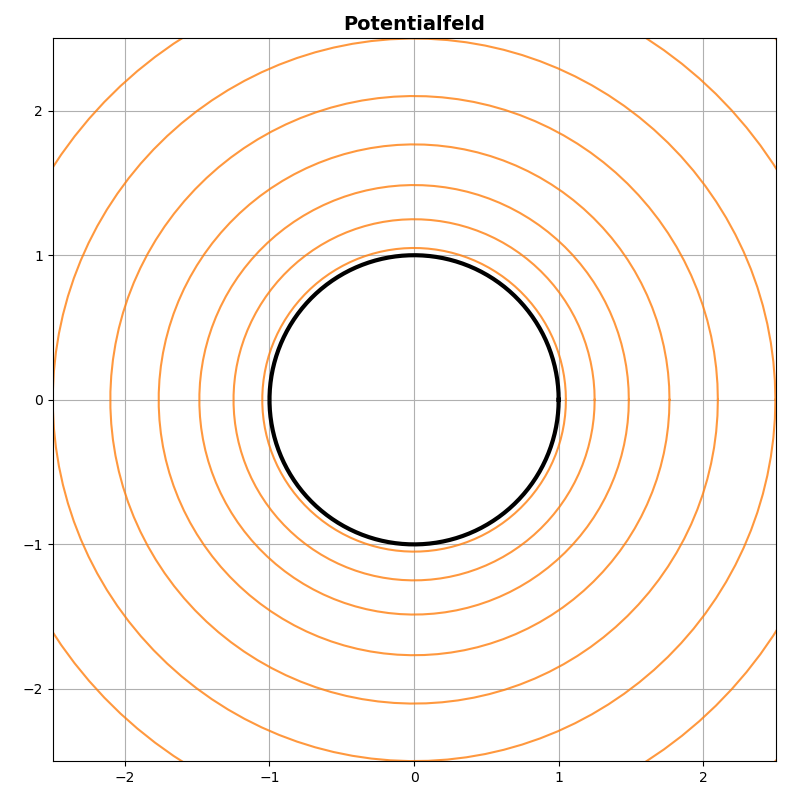
\includegraphics[width=0.9\linewidth]{papers/elektro/grafik/phi_feld_kreis.png}
	\label{elektro:figure:phi_feld}
	\caption[]{Es werden die Äquipotentiallinien dargestellt, um so näher die Linien beieinander liegen, desto höher ist das Potential, und somit auch das elektrische Feld. Der Rand des Kreises hat dabei ein beliebiges Potential gesetzt.}
\end{figure}


%\subsection{Äquipotentiallinien
%\label{elektro:subsection:Aequipotentiallinien}}
%Wie bereits erwähnt, sind die Äquipotentiallinien die Linien, auf denen das Potential $\varphi$ konstant ist.


% \subsection{Beispiel Einheitskreis
% \label{elektro:subsection:Einheitskreis-Beispiel}}
% In den Grafiken \ref{elektro:figure:e_feld} und \ref{elektro:figure:phi_feld} sind die Feldlinien und Äquipotentiallinien dargestellt ausserhalb des Einheitskreises.
% Der Rand des EInheitskreises wird in diesem Kapitel einfach als abgrenzung eines objekts angenommen.
% Das Feld ausserhalb ist dabei immer gleich egal wie hoch das potential ist oder ob einfach nur angenommen wird das der Einheitskreis als einzelne ladung angenommen wird.
% Theoretisch kann angenommen werden das der Kreis auf die Grösse eines Elektrons geschrumpft wird dabei würde das Feld immer noch gleich aussehen. 

\subsection{Zusammenhang zwischen E-Feld und Potential über komplexe Funktionen
\label{elektro:subsection:komplex}}
Das Ziel dieses Abschnitts ist, die Beziehung zwischen Äquipotentiallinien und dem elektrische Feld zu zeigen.
Die beiden Funktionen $\vec{E}$ und $\varphi$ können gemeinsam dargestellt werden.
Dabei wird ein wichtiger Zusammenhang klar: Die Potentiallinien und E-Feldlinien stehen immer senkrecht aufeinander.
Dies wird hier mit komplexen Funktionen erklärt, die in Kapitel \ref{chapter:holomorph} eingeführt wurden.
Dort werden auch die Cauchy-Riemann Gleichungen beschrieben, welche die Grundlage für die Beziehung zwischen den beiden Feldern bilden.
Wir bilden eine komplexe Funktion $f(z) = u(x,y) + iv(x,y)$, hierbei hängen Real- und Imaginärteil nur von den reellen Variablen x und y ab, also den zweidimensionalen Koordinaten unseres Abbildungssystems.
Der Realteil $u$ wird als elektrostatisches Feld definiert und ist nun eine Funktion von $x$ und $y$.
Der Imaginärteil $v$ ist das Potentialfeld.
Beide Funktionen erfüllen die Cauchy-Riemann Gleichungen, und sind daher holomorph. 
Es kann jetzt auch gezeigt werden, wieso die beiden Felder senkrecht aufeinander stehen.
Da diese Funktionen die Laplace-Gleichung 
\begin{equation}
	\Delta u = 0
	\label{elektro:equation:laplace}
\end{equation}
und 
\begin{equation}
	\Delta v = 0
\end{equation}
erfüllen,
kann, wenn eine der beiden bekannt ist, die jeweils andere Funktion sofort bestimmt werden.
Wenn zum Beispiel die Funktion $u$ des elektrischen Feldes bekannt ist, können wir schreiben:
\begin{equation}
	dv = \frac{\partial v}{\partial x}dx + \frac{\partial v}{\partial y} dy = 
	-\frac{\partial u}{\partial y}dx + \frac{\partial u}{\partial x}dy
\end{equation}
und diese Gleichung integrieren, um $v$ zu bestimmen.
Die beiden Vektoren
\begin{equation}
	\nabla{u} = \left(\frac{\partial u}{\partial x}, \frac{\partial u}{\partial y} \right)
\end{equation}
und 
\begin{equation}
	\nabla{v} = \left(\frac{\partial v}{\partial x}, \frac{\partial v}{\partial y} \right)
\end{equation}
stehen senkrecht aufeinander, das heisst sie sind normal zu einander:
\begin{equation}
	\vec{u} \cdot \vec{v} = 0.
\end{equation}
Das bedeutet, die beiden Funktionen $u(x,y)$ und $v(x,y)$ sind lokal senkrecht in ihren Schnittpunkten, 
ebenso wie das elektrische Feld und das Potentialfeld.


%\section{Komplexe Funktionen in der Elektrostatik
%\label{elektro:section:Funktionen-komplexer-Var}}
%Zur Erinnerung: Eine komplexe Zahl $z$ wird in kartesischen Koordinaten als Real- und Imaginärteil wie folgt dargestellt: $z = x + iy$.
%Eine komplexe Funktion $f(z) = u + iv$ kann aufgeteilt werden in zwei Funktionen $u = u(x,y)$ und $v = v(x,y)$, die von den realen Variablen $x$ und $y$ abhängig sind.
%Ein erstes Beispiel ist die Funktion $f(z) = z^{2}$.
%Da mit den Real- und Imaginärteilen wie gewohnt gerechnet werden kann, ergibt das Quadrieren: 
%\begin{equation}
%	(x+iy)^{2} = x^{2} - y^{2} + i2xy,
%\end{equation} 
%mit
%\begin{equation}
%	u(x,y) = x^{2} - y^{2}
%\end{equation} 
%und 
%\begin{equation}
%	v(x,y) = 2xy.
%\end{equation}

%\subsection{Holomorphe oder analytische Funktion
%\label{elektro:subsection:holomorph}}
%Die kontinuierlichen Funktionen $u(x,y)$ und $v(x,y)$ mit kontinuierlichen partiellen Ableitungen sind dann holomorph, wenn sie die Cauchy-Riemann Gleichungen
%\begin{equation}
%	\label{elektro:subsection:holomorph:Cauchy1}
%	\frac{\partial u}{\partial x} = \frac{\partial v}{\partial y}
%\end{equation}
%und 
%\begin{equation}
%\label{elektro:subsection:holomorph:Cauchy2}
%	\frac{\partial u}{\partial y} =
%	- \frac{\partial v}{\partial x}
%\end{equation}
%
%erfüllen.
%Holomorph bedeutet differenzierbar in jeder Ordnung und darstellbar als Exponentialreihe.
%Das Integral der Funktion entlang eines geschlossenen Weges in der komplexen Zahlenebene ist Null
%\begin{equation}
%	\oint f(z) \,dz = 0.
%\end{equation}
%\textcolor{red}{Streichen, auf Kapitel 1 und 2 verweisen}


%\subsection{Gausssches Gesetz
%\label{elektro:subsection:Gauss}}



%\subsection{Zusammenhang zwischen E-Feld und Potential
%\label{elektro:subsection:ephizusammenhang}}
%Etwas vorgreifend wird hier gezeigt, wie im Falle eines Kreises mathematisch von einem Potentialfeld $\varphi$ auf das elektrische Feld $\mathbf{E}$ geschlossen werden kann.
%Die Fläche außerhalb des Kreises wird als Potentialfeld beschrieben.

%
% teil1.tex -- Beispiel-File für das Paper
%
% (c) 2020 Prof Dr Andreas Müller, Hochschule Rapperswil
%
% !TEX root = ../../buch.tex
% !TEX encoding = UTF-8
%


\section{Riemannscher Abbildungssatz
\label{elektro:section:ReimannSatz}}
\kopfrechts{Riemannscher Abbildungssatz}

Georg Fridrich Bernhard Riemann (1826-1866) \textcolor{red}{cite from bibliography} war ein deutscher Mathematiker, der sich mit diversen Gebieten der Mathematik beschäftigte.
Auf vielen hat er bahnbrechende Ergebnisse erzielt, die bis heute von grosser Bedeutung sind, auch Einstein hat von seinen Theorien Gebrauch gemacht.
Der Riemannsche Abbildungssatz hat er erstmals als Skizze im Jahre 1851 in seiner Dissertation veröffentlicht. 
Erst später wurde der Satz von anderen Mathematikern formal bewiesen und in die Mathematik eingeführt. 
Es wird verschiedene Beweise für den Satz gefunden, die alle auf unterschiedlichen mathematischen Gebieten basieren.
Hier wird der verbreitetste Beweis vorgestellt, der auf dem Satz von Montel basiert, der die Existenz von konformen Abbildungen auf einfach zusammenhängende Gebiete beschreibt.
Beschriebt ist hier wörtlich gemeint, es gibt für den Riemannschen Abbildungssatz keine allgemeine Formel, die für alle Gebiete gilt, sondern nur einen Existenzbeweis einer Abbildung.
Dies bedeutet, dass es für jegliche Figuren eine Transformation existiert diese muss aber auf anderem Wege ermittelt werden dazu mehr in Abschnitt \ref{elektro:section:KreisTrafo}.

Im Allgemeinen ist unser Ziel ein Gebiet $G$ auf ein einfacheres Gebiet $G'$ abzubilden, um die Berechnung von Potential Feldern und elektrischen Feldern zu vereinfachen. 
Das ziel Gebiet $G'$ ist für uns der Einheitskreis, da für diesen die Formeln für das Potentialfeld $\varphi$ und das elektrische Feld $\mathbf{E}$ bereits bekannt sind. \textcolor{red}{Abschnitt verweis}

\subsection{Voraussetzungen
\label{elektro:subsection:RiemannVoraussetzungen}}
Zunächst müssen einpaar Voraussetzungen für den Riemannschen Abbildungssatz erfüllt sein, damit der Satz überhaupt angewendet werden kann.

\subsubsection{Einfach zusammenhängende Gebiete}
Das ursprüngliche Gebiet $G$ muss einfach zusammenhängend sein, das bedeutet, dass es keine Löcher in dem Gebiet gibt. 
Das Gebiet $G$ darf beliebig gross und beliebig geformt sein, solange es keine ausgeschnittene Bereiche enthält.
Zu dieser Definition gehört auch dazu, dass das Gebiet offen sein muss. Soll heissen der Rand von dem Gebiet gehört nicht zum Gebiet dazu.
Der Rand müsste separat betrachtet werden, wobei sich meistens herausstellt, dass der Rand sich brav mit verformt und die Abbildung auf dem Rand auch konform ist.
Es entstehe erst Abweichungen, wenn der Rand ausgefallene Fraktale bildet, dies ist bei uns nicht der Fall daher wird stets angenommen das der Rand analog zur Fläche verformt wird.

\subsubsection{Teilgebiete der komplexen Ebene}
$ G \subset \mathbb{C} $ muss gelten, dies bedeutet, dass $G$ ein Subset und nicht äquivalent zu $\mathbb{C}$ sein darf.
Für die komplette komplexe Ebene gilt der Riemannsche Abbildungssatz.
Wenn die gesamte komplexe Ebene auf den Einheitskreis abgebildet werden soll, dann müssten punkte die bereits im Innern des Einheitskreises liegen, unberührt bleiben und die, die ausserhalb liegen müssten auf bereits besetzte Punkte transformeirt werden. 
Die nächste Voraussetzung würde damit verletzt werden, die Bijektivität der Abbildung.

\subsubsection{Bijektive Abbildung}
Bijektiv bedeutet, dass alles eindeutig abgebildet wird, es gibt keine Punkte, die auf den gleichen Punkt abgebildet werden. 
Es geht also sowohl bei der Transformation sowie bei der Rücktransformation nichts an Information verloren.
Ansonsten würde eine Zweideutigkeit entstehen und die Abbildung wäre nicht mehr umkehrbar.


%
% teil2.tex -- Beispiel-File für teil2 
%
% (c) 2020 Prof Dr Andreas Müller, Hochschule Rapperswil
%
% !TEX root = ../../buch.tex
% !TEX encoding = UTF-8
%
\section{Der Kreis
\label{elektro:section:DerKreis}}
\kopfrechts{Der Kreis}
Bevor wir im nächsten Kapitel die Transformation von Kreisen betrachten, wollen wir uns mit den Eigenschaften des Kreises beschäftigen.
Der Kreis ist die einfachste und am besten verstandene Figur der Mathematik.
Elektrostatische Feldlinien und auch das Potential können leicht berechnet werden.
Für die elektrostatische Betrachtung dieses Kapitels ist der Kreis besonders geeignet.
Aufgrund der Rotationssymmetrie hängen sowohl das elektrische Feld $\vec{E}$ als auch das Potential $\varphi$ nur vom Abstand $r$ zum Mittelpunkt ab.

% \subsection{Radialsymmetrische Potentiale
% \label{elektro:subsection:RadialsymmetrischePotentiale}}
% Im Kreis ist das Potential radialsymmetrisch verteilt.
% Der Kreis kann eine Punktladung $Q$ darstellen oder eine Ladungsverteilung $\rho$, die sich auf der Kreisoberfläche befindet.
% % Der Kreis stellt eine Punktladung mit der Ladungsdichte $\rho$ dar.
% Da auch später immer von einer Ladungsverteilung $\rho$ auf verschiedenen Figuren ausgegangen wird, wird hier die Ladungsdichte $\rho$ als Ausgangspunkt genommen.
% Dank der Punktsymmetrie des Kreises ist das Potentialfeld durch Polarkoordinaten, die den Abstand $r$ und den Winkel $\varphi$ darstellen, vollständig beschrieben.  
% Im Abschnitt \ref{elektro:subsection:komplex} wurde gezeigt wie das Potentialfeld
% \begin{equation}
% 	\varphi = \int_{-\infty}^{\infty} \frac{\rho}{4\pi\varepsilon_0 r} dV
% 	\label{elektro:equation:potentialbegin}
% \end{equation}
% und das elektrische Feld $\vec{E}$ zusammenhängen.
% Es ergibt sich ein Kreislauf von Integralen, in welchem stets von einem Fall auf den anderen geschlossen werden kann und umgekehrt.
% Dazu muss jedoch eine dieser Formeln, die für den Kreis gültig ist, aufgestellt worden.
% Es braucht also einen Einstieg, durch den die Integralformel des elektrischen Feldes $\vec{E}$ gefunden werden kann. 
% Wie zuvor gezeigt, stellt der Kreis die Ladung dar und wir wollen das Potentialfeld ausserhalb des Kreises beschreiben.
% Dazu können wir das Integral des Potentials 
% \begin{equation}
%     \varphi = \int_{0}^{2\pi} \int_{r}^{\infty} \frac{\rho}{4\pi\varepsilon_0 r} r \, dr \, d\varphi
%     = \frac{\rho}{2\varepsilon_0} \int_{r}^{\infty} dr
%     = \frac{\rho}{2\varepsilon_0} [r]_{r}^{\infty}
%     = -\frac{\rho}{2\varepsilon_0} r
% \end{equation}
% von der Kreisoberfläche bis in die Unendlichkeit lösen.
% Die Abbildung dieser Formel ist in Abbildung \ref{elektro:figure:phi_feld} dargestellt.

% Verständnis: 
% Das Volumenelement wird zu $dV = r \, dr \, d\varphi $.
% Für beide Integrale wird die Integrationsgrenze von $0$ bis $2\pi$ für $\varphi$ und von $r$ bis $\infty$ für $r$ gewählt, da das Potentialfeld ausserhalb des Kreises beschrieben werden soll und dies um die gesamten $2\pi$ des Kreises.

%%%

\subsection{Radialsymmetrie von $\vec{E}$-Feld und dem Potential $\varphi$
\label{elektro:subsection:Radialsymmetrie}}

Für die zweidimensionale Betrachtung wird ein kreisförmiger Leiter mit Radius $R$ betrachtet.
Aufgrund der Rotationssymmetrie hängt das elektrische Feld ausserhalb des Kreises nur vom Abstand $r$ zum Mittelpunkt ab und zeigt radial nach aussen.
Die Ladung des Leiters wird durch die Ladung pro Längeneinheit $\rho$ beschrieben.
Dabei bezeichnet $\rho$ die Ladung pro Längeneinheit senkrecht zur betrachteten Ebene und hat die Einheit $\mathrm{C/m}$.
Gesucht ist nun das elektrische Feld an einem Punkt ausserhalb des Leiters.
Da jeder Punkt mit demselben Abstand $r$ vom Mittelpunkt aufgrund der Symmetrie dieselbe Feldstärke besitzt, kann ein konzentrischer Kreis mit Radius $r>R$ betrachtet werden.
Das Gausssche Gesetz bezieht sich auf eine geschlossene Fläche.
Da hier nur ein zweidimensionaler Querschnitt dargestellt wird, wird der Kreis gedanklich um eine beliebige Länge $\ell$ senkrecht zur Zeichenebene erweitert.
Die eingeschlossene Ladung beträgt dann $\rho \ell$.
Auf der seitlichen Fläche besitzt das elektrische Feld überall denselben Betrag $E(r)$ und zeigt senkrecht nach aussen. Damit ergibt sich aus dem Gaussschen Gesetz

\begin{equation}
    E(r)\,2\pi r\,\ell = \frac{\rho\,\ell}{\varepsilon_0}.
\end{equation}

Die beliebig gewählte Länge $\ell$ kürzt sich heraus. Für das elektrische Feld ausserhalb des Kreises folgt somit
\begin{equation}
    \vec{E}(r)
    =
    \frac{\rho}{2\pi\varepsilon_0 r}\hat{r}.
    \label{elektro:equation:efeld_radial}
\end{equation}
Das elektrische Feld beschreibt, wie stark und in welche Richtung eine positive Probeladung an einem bestimmten Ort beschleunigt würde.
Das Potential beschreibt dagegen die zugehörige potentielle Energie pro Ladung.
Sind zwei Punkte durch das elektrische Feld verbunden, ergibt sich ihre Potentialdifferenz aus dem Integral des Feldes entlang des Weges.
Als Referenz wird hier die Oberfläche des Leiters bei $r=R$ gewählt.
Damit gilt
\begin{equation}
    \varphi(r)-\varphi(R)
    =
    -\int_R^r \vec{E}\cdot d\vec{r}.
\end{equation}
Da das Feld radial verläuft, kann das zuvor bestimmte elektrische Feld eingesetzt werden:
\begin{equation}
\begin{aligned}
    \varphi(r)-\varphi(R)
    &=
    -\int_R^r
    \frac{\rho}{2\pi\varepsilon_0 r'}\,dr'
    \\[1mm]
    &=
    -\frac{\rho}{2\pi\varepsilon_0}
    \ln\left(\frac{r}{R}\right).
\end{aligned}
\end{equation}
Für den Einheitskreis gilt $R=1$.
Wird das Potential auf der Kreisoberfläche auf $\varphi(1)=0$ gesetzt, vereinfacht sich die Gleichung zu
\begin{equation}
    \varphi(r)
    =
    -\frac{\rho}{2\pi\varepsilon_0}\ln(r).
    \label{elektro:equation:potential}
\end{equation}


%%%%

\subsection{Kreisspiegelung
\label{elektro:subsection:Kreisspiegelung}}

Damit man sich die Kreisspiegelung vorstellen kann, wird der Kreisrand als Spiegeloberfläche angenommen.
Somit wird jeder Punkt ausserhalb des Kreises, auch die Unendlichkeit, in das Innere des Einheitskreises gespiegelt.
Analog dazu wird alles innerhalb des Einheitskreises nach aussen gespiegelt, wobei der Ursprung auf alle Seiten in die Unendlichkeit gespiegelt wird.

Diese Transformation wird hier nur gezeigt, weil durch diese Transformation die Wahl der Integralgrenzen im Abschnitt \ref{elektro:subsection:Radialsymmetrie} erklärt werden kann.
Es kann vom Mittelpunkt zum Kreisrand oder vom Kreisrand bis in die Unendlichkeit integriert werden und mit einer einfachen Kreisspiegelung im Komplexen vom einen zum anderen Fall übergegangen werden.
Mathematisch wird die Kreisspiegelung durch die Transformation
Mathematisch wird die Kreisspiegelung durch die Transformation
\begin{equation}
    z \mapsto \frac{1}{\overline{z}}
\end{equation}
beschrieben, wie im Kapitel \ref{chapter:geradlinig} erklärt wird. 

% \subsection{Zusammenhang zwischen $\vec{E}$-Feld und Potential
% \label{elektro:subsection:ephizusammenhang}}
% Anhand des Beispiels des Einheitskreises wird hier gezeigt, wie von einem Potentialfeld $\varphi$ auf das elektrische Feld $\vec{E}$ geschlossen werden kann, wie im Abschnitt \ref{elektro:subsection:Einheitskreis-Beispiel} behauptet wird.

% Unser Ausgangspunkt ist das elektrische Feld $\vec{E}$, das durch die Umformung zu zylindrischen Koordinaten auf $ \vec{E} = \frac{\rho}{2\pi\varepsilon_0 r} \hat{r} $ vereinfacht werden kann.
% Wird dies in die Formel \eqref{equation:Potential} eingesetzt, so ergibt sich das Potentialfeld 
% \begin{equation}
%     \varphi = - \int_{1}^{k} \frac{\rho}{2\pi\varepsilon_0 r} \hat{r} \cdot d\mathbf{r}
%     = - \frac{\rho}{2\pi\varepsilon_0}\vert ln(k) \vert_{1}^{r}
%     = - \frac{\rho}{2\pi\varepsilon_0} \operatorname{ln}(r).
%     \label{elektro:equation:potential}
% \end{equation}
% Ist nun das elektrische Feld bekannt, kann daraus auch das elektrische Potential berechnet werden.
% % Kontinuierlich kann auch vom Potentialfeld $\varphi$ auf das elektrische Feld $\mathbf{E}$ geschlossen weerden indem die Formel die sich aus dem soeben ausgeführen Integrals umgestellt wird. 
% Der Rückschluss vom Potentialfeld $\varphi$ auf das elektrische Feld $\vec{E}$ ist über die Laplace-Gleichung \ref{elektro:subsection:Laplace} möglich.
% Es muss konsistent in zylindrischen Koordinaten gearbeitet werden, damit die Ableitung des Potentials $\varphi$ nach $r$ das elektrische Feld $\vec{E}$
% \begin{equation}
%     \vec{E} = - \nabla \varphi = - \frac{\partial}{\partial r} \left( - \frac{\rho}{2\pi\varepsilon_0} \operatorname{ln}(r) \right) = \frac{\rho}{2\pi\varepsilon_0 r} \hat{r}
%     \label{elektro:equation:efeld}
% \end{equation}
% ergibt.
% Hiermit ist gezeigt, dass die Integrale in einem Kreislauf miteinander verbunden sind und von einem zum anderen geschlossen werden kann.

\subsection{Komplexe Darstellung}

Das zuvor bestimmte radialsymmetrische elektrische Feld kann nun komplex dargestellt werden.
Dabei bezeichnet $\rho$ weiterhin die Ladung pro Längeneinheit senkrecht zur betrachteten Ebene.

Für Punkte ausserhalb des Kreises mit $r>R$ gilt
\begin{equation}
    \vec{E} = \frac{\rho}{2\pi\varepsilon_0 r}\hat{r}.
\end{equation}
Mit
\begin{equation}
    \hat{r}
    =
    \frac{x}{r}\hat{x}
    +
    \frac{y}{r}\hat{y}
\end{equation}
und $r^2=x^2+y^2$ kann das elektrische Feld in kartesischen Koordinaten als
\begin{equation}
\begin{aligned}
    \vec{E}
    &=
    \frac{\rho}{2\pi\varepsilon_0 r}
    \left(
        \frac{x}{r}\hat{x}
        +
        \frac{y}{r}\hat{y}
    \right)
    \\[2mm]
    &=
    \frac{\rho}{2\pi\varepsilon_0}
    \left(
        \frac{x}{x^2+y^2}\hat{x}
        +
        \frac{y}{x^2+y^2}\hat{y}
    \right)
\end{aligned}
\end{equation}
geschrieben werden.
Damit ergeben sich die Komponenten des elektrischen Feldes zu
\begin{equation}
    E_x = \frac{\rho}{2\pi\varepsilon_0}\frac{x}{x^2+y^2}\quad\text{und}\quad
    E_y = \frac{\rho}{2\pi\varepsilon_0}\frac{y}{x^2+y^2}.
\end{equation}
Um die beiden Feldkomponenten in einer komplexen Funktion zusammenzufassen, wird die Notation
\begin{equation}
    \mathcal{E}(z)=E_x-iE_y
\end{equation}
verwendet.
Damit folgt
\begin{equation}
    \mathcal{E}(z) = \frac{\rho}{2\pi\varepsilon_0}\frac{x-iy}{x^2+y^2}.
\end{equation}
Für $z=x+iy$ gilt
\begin{equation}
\begin{aligned}
    \frac{1}{z}
    &=
    \frac{1}{x+iy}
    \\[2mm]
    &=
    \frac{x-iy}{(x+iy)(x-iy)}
    \\[2mm]
    &=
    \frac{x-iy}{x^2+y^2}.
\end{aligned}
\end{equation}
Damit kann das elektrische Feld kompakt als
\begin{equation}
    \boxed{
        \mathcal{E}(z) = \frac{\rho}{2\pi\varepsilon_0}\frac{1}{z}
    }
\end{equation}
geschrieben werden.

Auch das in Abschnitt \ref{elektro:subsection:Radialsymmetrie} bestimmte Potential kann mit der komplexen Koordinate $z$ dargestellt werden.
Da $r=|z|$ gilt, folgt für einen Kreis mit Radius $R$
\begin{equation}
    \varphi(z)
    = -\frac{\rho}{2\pi\varepsilon_0}\ln\left(\frac{|z|}{R}\right).
\end{equation}
Für den Einheitskreis mit $R=1$ und $\varphi(1)=0$ vereinfacht sich dies zu
\begin{equation}
    \boxed{
        \varphi(z) = -\frac{\rho}{2\pi\varepsilon_0}\ln|z|
    }.
\end{equation}
Das Potential $\varphi(z)$ bleibt dabei eine reellwertige Funktion.
Die komplexe Schreibweise wird verwendet, weil sich das elektrische Feld $\mathcal{E}(z)$ dadurch als Funktion der komplexen Koordinate $z$ darstellen und später mit komplexen Abbildungen transformieren lässt.
%
% teil3.tex -- Beispiel-File für Teil 3
%
% (c) 2020 Prof Dr Andreas Müller, Hochschule Rapperswil
%
% !TEX root = ../../buch.tex
% !TEX encoding = UTF-8
%

\section{Komplexe Transformationen auf den Kreis
\label{elektro:section:KreisTrafo}}
\kopfrechts{Kreis Transformationen}

Im Abschnitt \ref{elektro:section:RiemannSatz} wurden die Voraussetzungen für die Anwendung des riemannschen Abbildungssatzes beschrieben.
Dabei wurde erwähnt, dass es keine allgemeine Formel für die Abbildung von beliebigen Gebieten auf den Einheitskreis gibt.
Daher suchen wir nach einer Methode, die uns erlaubt, die Abbildung für beliebige Gebiete zu finden, damit wir die Feldberechnungen vereinfachen können.

Unser Ziel ist es bekanntlich, Berechnungen anhand des Einheitskreises durchzuführen, da wir dort die Feldgleichungen bereits kennen. 
(Siehe Gleichung \eqref{elektro:equation:potential} und \eqref{elektro:equation:efeld}).
Für eine solche Transformation gibt es mathematisch mehrere Ansätze, die zu einer Lösung führen.
Es wird hier über das Schwarz-Christoffel-Verfahren und über den numerischen Ansatz berichtet, der auf der Finite-Elemente-Methode basiert.
\textcolor{red}{Quelle}

% Hier wird der Ansatz über die Schwarz-Christoffel-Transformationen vorgestellt, die auf einem approximativen Integrationsverfahren basiert.

\subsection{Schwarz-Christoffel-Transformation
\label{elektro:section:SchwarzChristoffel}}
Die Schwarz-Christoffel-Transformation ist ein Verfahren, um den Einheitskreis auf ein Polygon abzubilden. 
Es geht darum, den Rand des Einheitskreises auf den Rand des Polygons abzubilden, sodass die Abbildung konform ist $f: D \rightarrow P $.
Wenn der Einheitskreis $D = {w \in C ; \vert w \vert < 1}$ ist, dann ist der Rand des Einheitskreises $\vert w \vert = 1$, die Bedingung wird nun verwendet um Punkte auf dem Rand des Einheitskreises festzulegen, die auf die Ecken des Polygons abgebildet werden.
Die Punkte auf dem Einheitskreis, die so genannten \emph{Prevertices}, werden als $w_1, w_2, ..., w_n$ bezeichnet, dabei gilt: $\vert w_n \vert = 1$.
Die Prevertices werden als komplexe Zeiger dargestellt, $w_k = e^{\i \theta_k} $.
Die Ecken des Polygons werden als $z_1, z_2, ..., z_n$ bezeichnet.
Und jetzt wird die Funktion $f(w_n) = z_n$ gesucht, welche die $w_n$ auf die $z_n$ abbildet. \textcolor{red}{Laufvariable k oder n ?}
Die Konstruktion beruht auf den bekannten Innenwinkeln der Ecken des Polygons, die als $\alpha_1, \alpha_2, ..., \alpha_n$ bezeichnet werden, und auf den Seitenlängen des Polygons, $L_k = \vert z_{k+1} - z_k \vert$.

Als erster Schritt in der Berechnung wird nun die Ableitung der Schwarz-Christoffel Formel verwendet, da vorerst nur die Richtungsänderung an den Ecken des Polygons von Bedeutung ist
\begin{equation}
	f'(w) = C \prod_{k=1}^{n} \biggl(1-\frac{w}{w_k}\biggr)^{\alpha_k-1}.
	\label{elektro:equation:SchwarzChristoffelDerivative}
\end{equation}
$C$ ist eine komplexe Konstante, die später bestimmt wird und $\alpha_k$ ist bereits bekannt.
Daher fehlen nur noch die Prevertices $w_k$.
Diese werden durch die Seitenlängen des Polygons aufgespürt, da durch die Konformität der Abbildung die Seitenlängen des Polygons erhalten bleiben müssen. 
Damit ohne den Faktor C vorgegangen werden kann, wird das Verhältnis zweier benachbarter Seiten gebildet.
Damit entsteht das folgende Gleichungssystem für die Prevertices $w_k$
\begin{equation}
	\frac{L_k}{L_1} = \frac{\bigg\vert \int_{w_k}^{w_{k+1}} \prod_{j=1}^{n}(1-\frac{w}{w_j})^{\alpha_j-1} dw \bigg\vert}{\bigg\vert \int_{w_1}^{w_2} \prod_{j=1}^{n}(1-\frac{w}{w_j})^{\alpha_j-1} dw \bigg\vert}.
	\label{elektro:equation:SchwarzChristoffelPrevertices}
\end{equation}
Dieses Gleichungssystem ist nichtlinear, weswegen es immer von einem Computer gelöst wird, indem er die Prevertices solange hin und her schiebt bis die Seitenlängenverhältnisse übereinstimmen.
Die gesamte Abbildung wird durch das Integral aller Teile der Ableitung gebildet
\begin{equation}
	f(w) = A + C \int_{w_0}^{w} \prod_{k=1}^{n}(1-\frac{\zeta}{w_k})^{\alpha_k-1} d\zeta,
	\label{elektro:equation:SchwarzChristoffel}
\end{equation}
wobei die Integrationsgrenze $w_0$ auf einen beliebigen Punkt des Einheitskreises gesetzt werden kann, da die Abbildung bis auf eine Translation eindeutig ist.
In diesem Anwendungsfall ist vielleicht aufgefallen, dass immer das Feld ausserhalb des Polygons betrachtet wird, daher muss hier noch die feine Unterscheidung gemacht werden, dass die Aussenwinkel betrachtet werden müssen. 
Dazu kommt dass die Fläche des Einheitskreises von innen nach aussen gestülpt werden muss, was wie in Abschnitt \ref{elektro:subsection:Kreisspiegelung} beschrieben durch die Kreisspiegelung erreicht wird. 
In der Gleichung
\begin{equation}
	f(w) = A + C \int_{w_0}^{w} \frac{1}{{\zeta}^2}\prod_{k=1}^{n}(1-\frac{\zeta}{w_k})^{-\alpha_k-1} d\zeta
	\label{elektro:equation:SchwarzChristoffelExterior}
\end{equation}
kommen weitere Faktoren hinzu: \ref{elektro:equation:SchwarzChristoffelExterior}:
\begin{itemize}
	\item $\frac{1}{\zeta^2}$: Dieser Faktor sorgt dafür dass der Ursprung des Kreises nach $\infty$ gefördert wird.
	\item $-\alpha_k-1$: Das Minus vor dem Exponenten sorgt dafür dass die Aussenwinkel des Polygons betrachtet werden.
\end{itemize}

Um das Beschriebene zu veranschaulichen sind in Abbildung \ref{elektro:figure:SchwarzChristoffel_erklaerung} die Prevertices $w_n$, die Ecken des Polygons $z_n$ und die Winkel $\alpha_k$ eingezeichnet.


\begin{figure}
	\centering
	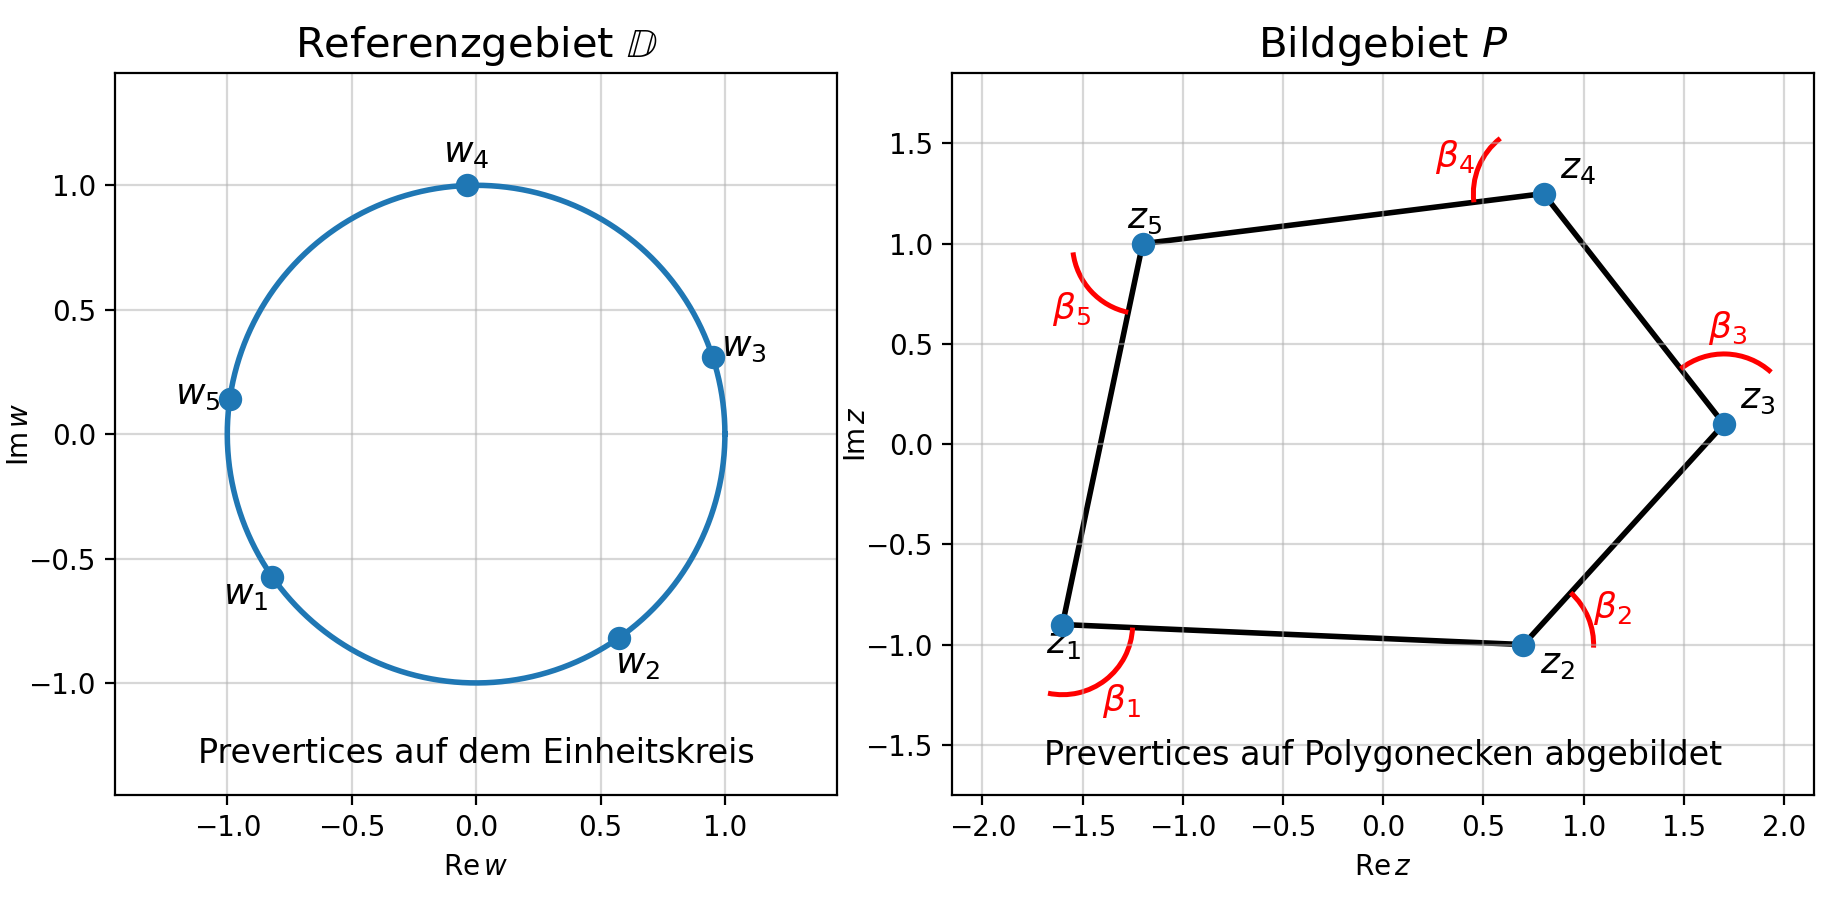
\includegraphics[width=0.9\textwidth]{papers/elektro/grafik/SC_trafo_erklaerung.png}
	\caption{Prevertices, Ecken und $\alpha_{k}$ abgebildet}
	\label{elektro:figure:SchwarzChristoffel_erklaerung}
\end{figure}



% \subsection{MATLAB Toolbox für Schwarz-Christoffel-Transformationen}
% \label{papers:elektro:subsection:sc-toolbox}


\subsection{Beispiel: Dreieck auf Kreis}
Ein dreieckige Kontur eines ladungsbehafteten Objektes kann als einfaches Beispiel viele Effekte der Transformation zeigen.
Mit der Schwarz-Christoffel Transformation kann nun der Einheitskreis so transformiert werden, dass deren Rand die Form unseres Dreiecks annimmt und damit ein Feld berechnet werden kann, das exakt die Form des Dreiecks hat.
Für die Berechnung der Prevertices und alle anderen Parameter wird das MATLAB-Tool benutzt, das in Abschnitt \ref{papers:elektro:subsection:sc-toolbox} beschrieben wurde. 
%\textcolor{red}{ist die Beschreibung des Tools überhaupt nötig ?}
Danach wird die Transformation angewendet, wodurch das Feld so herauskommt wie in Abbildung \ref{elektro:figure:SC_triag_trafo} dargestellt.

\begin{figure}
	\centering
	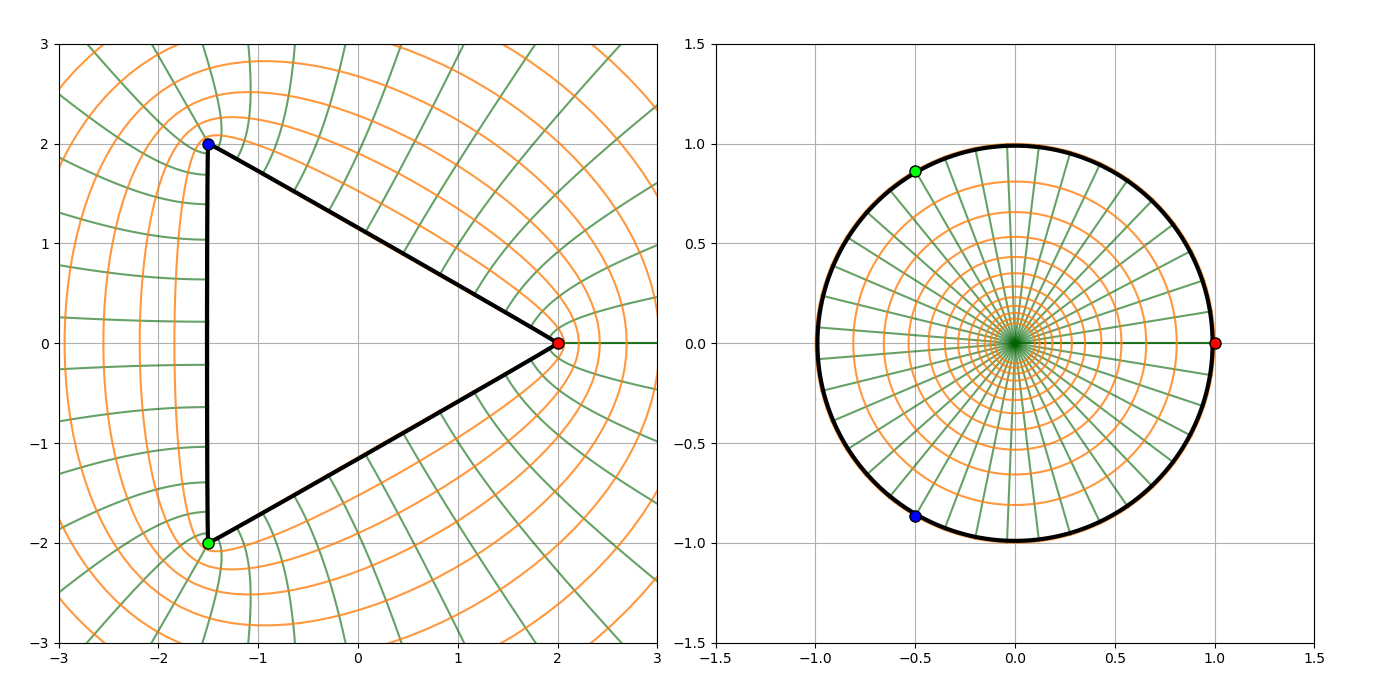
\includegraphics[width=0.9\textwidth]{papers/elektro/grafik/SC_trafo_triag.png}
	\caption{Schwarz-Christoffel transformiertes Polygon auf das Innere des Einheitskreises}
	\label{elektro:figure:SC_triag_trafo}
\end{figure}

In Abbildung \ref{elektro:figure:SC_triag_trafo} ist zu sehen, wie die Feldlinien auf der Oberfläche des Dreiecks senkrecht aufkommen und sich im Raum ausbreiten und dabei auch die Potentiallinen immer senkrecht kreuzen.
Es sind auch die Prevertices auf dem Einheitskreis eingezeichnet, welche diejenigen Punkte markieren, die exakt auf die Ecken des Dreiecks transformiert werden.
Die Farben zeigen welcher Punkt auf welche Ecke transformiert wird. 
Dabei fällt auf, dass die Prevertices nicht intuitiv in derselben Richtung wie die Ecken des Dreiecks angeordnet sind, sondern in entgegengesetzter Richtung. 
Dies ist auf eine Regel innerhalb von Matlab zurückzuführen, die besagt dass die Fläche die bearbeitet wird, im mathematischen Sinn, immer auf der linken Seite der Kurve liegen muss.
Wenn die Laufvariable des Integrals sich auf der Kurve fortbewegt, muss die Fläche, die bearbeitet wird, immer auf der linken Seite liegen.
Mit einem kleinen gedanklichen Experiment kann nun festgestellt werden, dass die Verlaufsrichtung auf dem Dreieck im Uhrzeigersinn sein muss und beim Einheitskreis gegen den Uhrzeigersinn.

\subsection{Komplexere Geometrie}
Als etwas komplexere Geometrie mit mehreren Ecken, darunter auch einige, die einen Innenwinkel grösser als $180^{\circ}$ haben, wird ein hufeisenförmiges Polygon gezeigt.
\begin{figure}
	\centering
	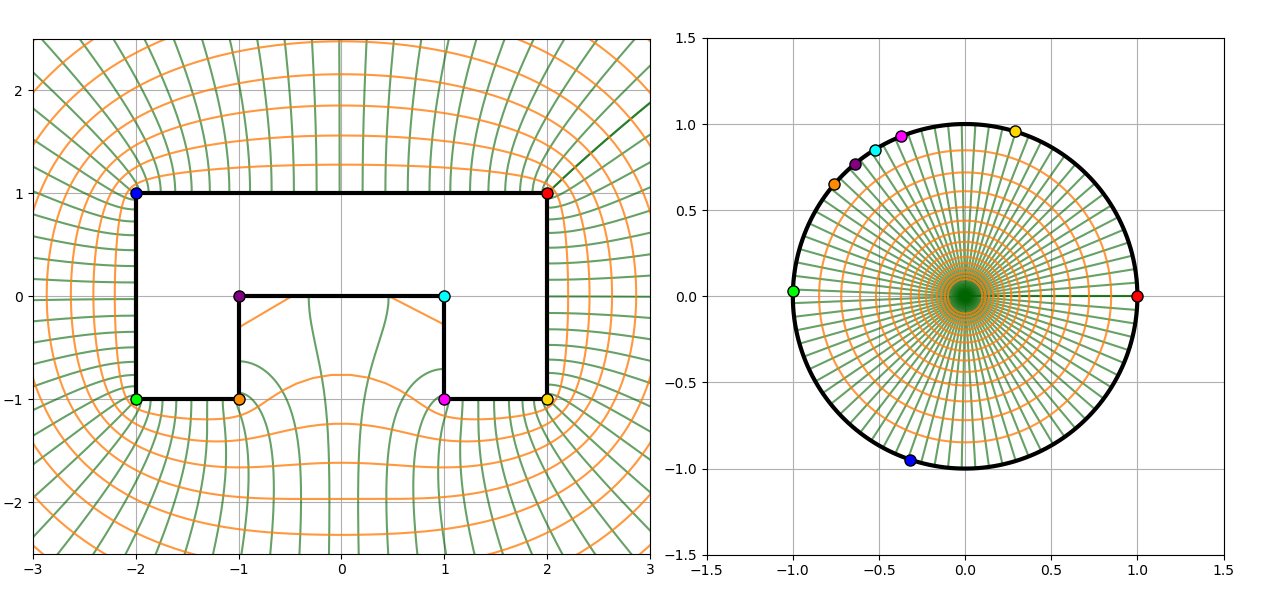
\includegraphics[width=0.9\linewidth]{papers/elektro/grafik/SC_trafo_huf.png}
	\caption{Schwarz-Christoffel transformiertes Polygon auf das Innere des Einheitskreises}
	\label{elektro:figure:SC_huf_trafo}
\end{figure}

In Abbildung \ref{elektro:figure:SC_star_trafo} sind drei verschiedene Winkel zu finden, die alle eine andere Konzentration an Feldlinen aufweisen die senkrecht dort aufkommen.
Bei spitzen winkeln ist zu sehen, dass die Feldlinen näher beieinander sind und bei den stumpferen oder sogar überstumpfen Winkeln sieht man, dass die Feldlinen weiter auseinander liegen.
Dies ist auf die Ladungsverteilung auf dem Objekt zurückzuführen:
Bei spitzeren Winkeln hat es weniger Platz zwischen den beiden Kanten und Ladungsträger drücken die vor ihnen liegenden Ladungsträger näher zusammen, was zu einer höheren Ladungsdichte an den Spitzen führt.
Bei den stumpferen Winkeln ist es genau umgekehrt, dort hat es mehr Platz und die Ladungsträger können sich weiter auseinander verteilen (was genau das ist, was Ladungsträger mit gleicher Polarität am liebsten tun). 
Genau wie die $E$-Feldlinen, die sich gegenseitig abstossen und sich so weit wie möglich voneinander entfernen.

\begin{figure}
	\centering
	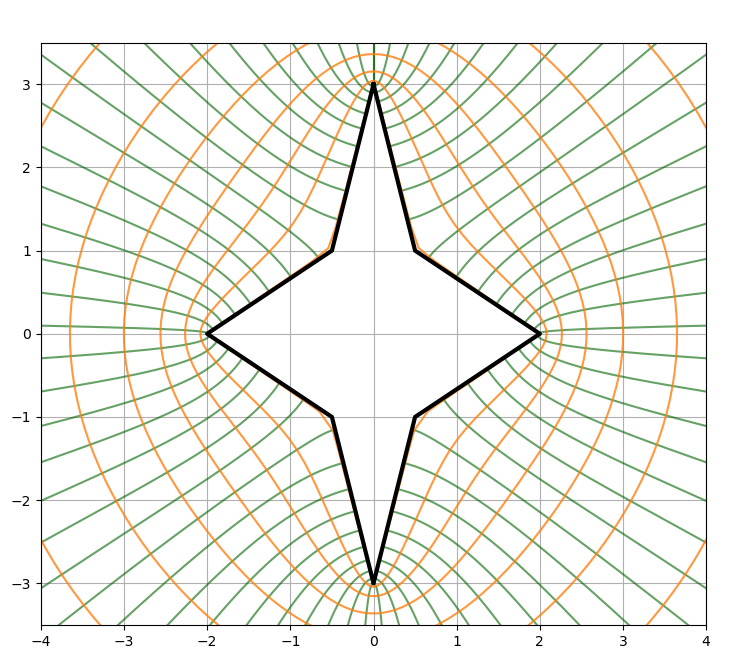
\includegraphics[width=0.9\linewidth]{papers/elektro/grafik/SC_trafo_star.png}
	\caption{Sternförmige Kontur mit verschiedenen Innenwinkeln}
	\label{elektro:figure:SC_star_trafo}
\end{figure}

Diese Spitzeneffekte sind nicht auf die Elektrostatik beschränkt, sondern kommen in allen Bereichen der Physik vor.
In der Mechanik ist es das gleiche Prinzip, dass sich Kräfte an den Spitzen von Objekten konzentrieren und dort zu einer höheren Belastung führen.
In Abbildung \ref{elektro:figure:mech_triag} ist ein Beispiel davon zu sehen, wie sich die Kräfte an den Spitzen eines Dreiecks konzentrieren.

\begin{figure}
	\centering
	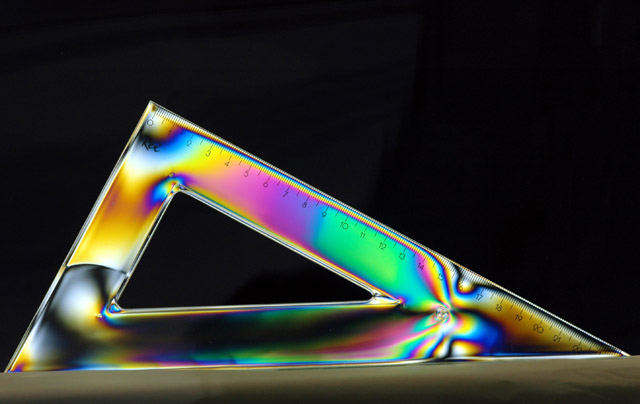
\includegraphics[width=0.9\linewidth]{papers/elektro/grafik/mech_triag.png}
	\caption{Kraftkonzentration an den Spitzen eines Dreiecks}
	\cite[Bild Quelle]{elektro:mech_triag}
	\label{elektro:figure:mech_triag}
\end{figure}

%\input{papers/elektro/00_grafiken.tex}

\printbibliography[heading=subbibliography]
\end{refsection}

%Vektorfelder einheitlich als \vec{E} schreiben
